\documentclass{jsarticle}
\usepackage[dvipdfmx]{graphicx}
\usepackage{subcaption}
\captionsetup[figure]{justification=centering}
\captionsetup[table]{justification=centering}
\usepackage[ipa]{pxchfon}
\usepackage{float}
\usepackage[margin=20truemm]{geometry}


\begin{document}
\title{{\vspace*{-10mm}}{\LARGE 0706課題}}
\author{\large 千葉工業大学 先進工学部 未来ロボティクス学科 \vspace*{4mm}\\20C1015 今井悠月}
\date{}
\maketitle\vspace*{10mm}
\vspace*{-10mm}

\section*{問}
本日学んだ予見制御を用いた歩行パターン生成を応用して, octaveを使用して歩行パターンを生成せよ.

\section*{解答}

\begin{figure}[H]
  \centering
   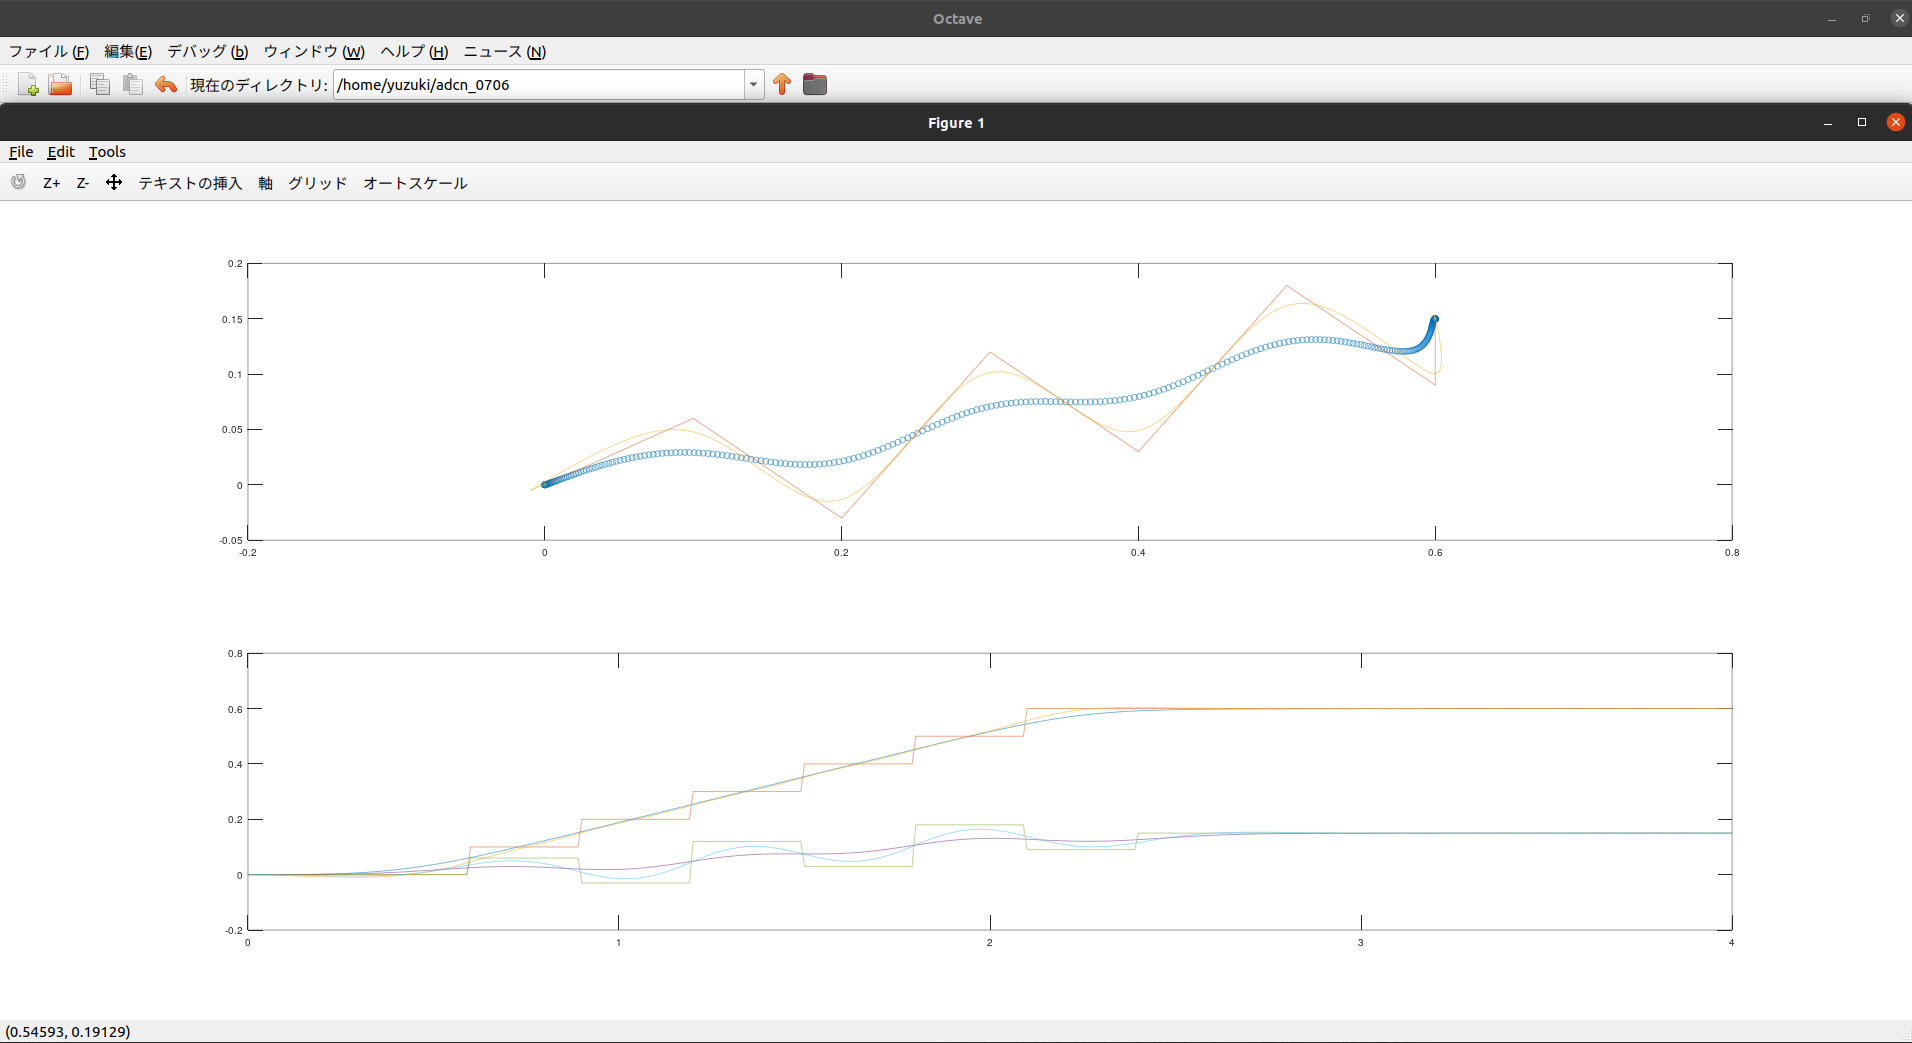
\includegraphics[scale=0.27]{./fig/1.png}
   \caption{実行結果のグラフ}
\end{figure}

\begin{figure}[H]
  \centering
   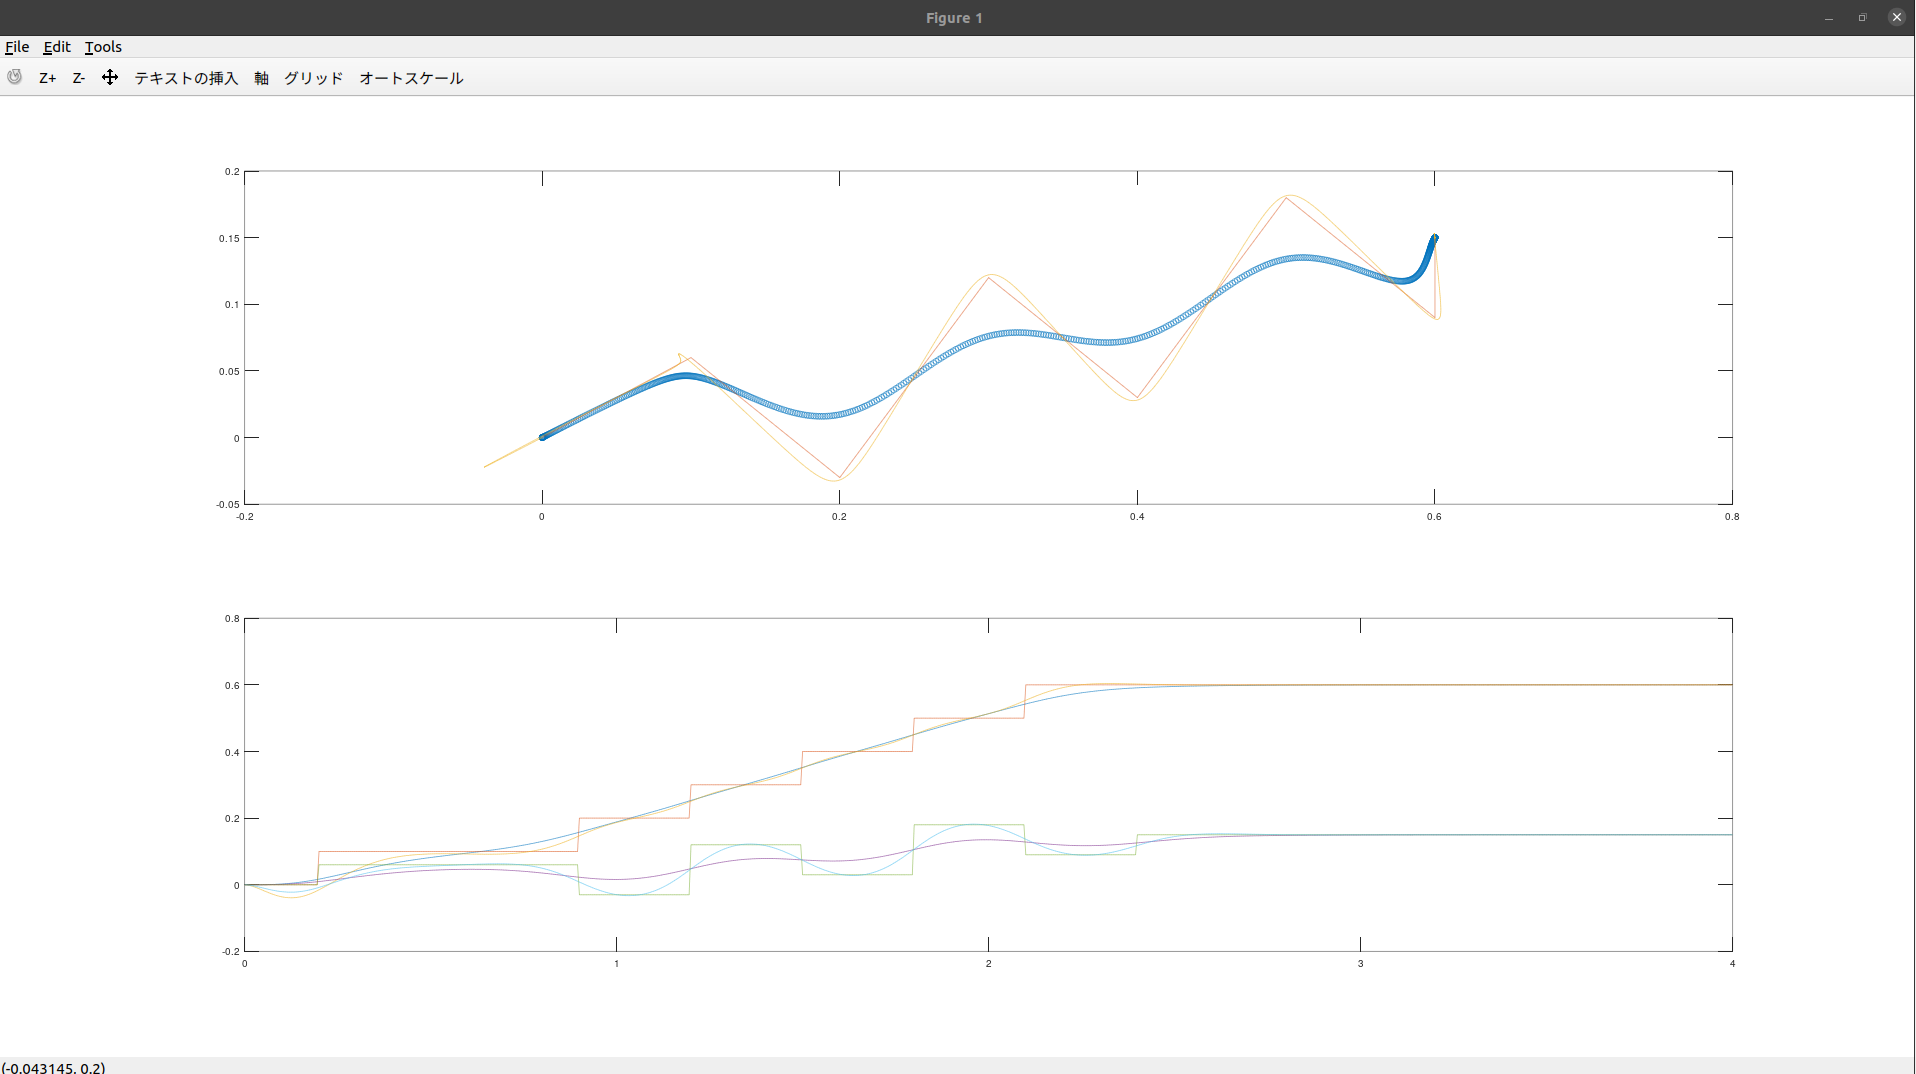
\includegraphics[scale=0.27]{./fig/2.png}
   \caption{条件を変えて計算した結果のグラフ}
\end{figure}

\subsection*{変更した条件と簡単なコメント}
mファイル中の5行目の foot の足の着地時間(s) を 0.6 → 0.2 に変更\\
\hspace*{1zw}また, サンプリングタイム dt を 0.01 → 0.005 に変更\\
\hspace*{1zw}デフォルトの値で実行した結果のグラフよりも, 理想的なZMPの軌道に沿うように実際のZMPが変動した.
\end{document}